% Copyright © 2012 Martin Ueding <dev@martin-ueding.de>
%
\documentclass[11pt, ngerman, fleqn]{article}

\usepackage[a4paper, left=3cm, right=2cm, top=2cm, bottom=2cm]{geometry}
\usepackage[activate]{pdfcprot}
\usepackage[cdot, squaren]{SIunits}
\usepackage[iso]{isodate}
\usepackage[parfill]{parskip}
\usepackage[T1]{fontenc}
\usepackage[utf8]{inputenc}
\usepackage{amsmath}
\usepackage{amsthm}
\usepackage{babel}
\usepackage{color}
\usepackage{lastpage}
\usepackage{commath}
\usepackage{epstopdf}
\usepackage{fancyhdr}
\usepackage{graphicx}
\usepackage{hyperref}
\usepackage{setspace}
\usepackage{tikz}

\usepackage[charter, greekuppercase=italicized]{mathdesign}


\usetikzlibrary{arrows}
\usetikzlibrary{intersections}

\definecolor{darkblue}{rgb}{0,0,.5}
\definecolor{darkgreen}{rgb}{0,.5,0}

\hypersetup{
	breaklinks=false,
	citecolor=darkgreen,
	colorlinks=true,
	linkcolor=black,
	menucolor=black,
	urlcolor=darkblue,
}

\setlength{\columnsep}{1.5cm}

\DeclareMathOperator{\arcsinh}{arsinh}
\DeclareMathOperator{\arsinh}{arsinh}
\DeclareMathOperator{\asinh}{arsinh}
\DeclareMathOperator{\card}{card}
\DeclareMathOperator{\diam}{diam}

\newcommand{\dalambert}{\mathop{{}\Box}\nolimits}
\newcommand{\divergence}[1]{\inner{\vnabla}{#1}}
\newcommand{\ee}{\mathrm e}
\newcommand{\emesswert}{\del{\messwert \pm \messwert}}
\newcommand{\e}[1]{\cdot 10^{#1}}
\newcommand{\fehlt}{\textcolor{red}{Hier fehlen noch Inhalte.}}
\newcommand{\half}{\frac 12}
\newcommand{\ii}{\mathrm i}
\newcommand{\inner}[2]{\left\langle #1, #2 \right\rangle}
\newcommand{\laplace}{\mathop{{}\bigtriangleup}\nolimits}
\newcommand{\messwert}{\textcolor{blue}{\square}}
\newcommand{\punkte}{\textcolor{white}{xxxxxxx}}
\newcommand{\tens}[1]{\boldsymbol{#1}}
\newcommand{\vnabla}{\vec \nabla}
\renewcommand{\vec}[1]{\boldsymbol{#1}}

\newcommand{\themodul}{physik311}
\newcommand{\thegruppe}{Gruppe 3 -- Matthias Rehberger}
\newcommand{\theuebung}{3}

\pagestyle{fancy}

\fancyfoot[C]{\footnotesize{\thegruppe}}
\fancyfoot[L]{\footnotesize{Martin Ueding}}
\fancyfoot[R]{\footnotesize{Seite \thepage\ / \pageref{LastPage}}}
\fancyhead[L]{\themodul{} -- Übung \theuebung}

\setcounter{section}{12}

\def\thesubsection{\thesection\alph{subsection}}

\title{\themodul{} -- Übung \theuebung \\ \vspace{0.5cm} \large{\thegruppe}}

\author{Martin Ueding \\ \small{\href{mailto:mu@uni-bonn.de}{mu@uni-bonn.de}}}

\begin{document}

\maketitle

\begin{table}[h]
	\centering
	\begin{tabular}{l|c|c|c|c|c}
		Aufgabe & \ref{1} & \ref{2} & \ref{3} & \ref{4} & $\sum$   \\
		\hline
		Punkte & \punkte & \punkte & \punkte & \punkte & \punkte
	\end{tabular}
\end{table}

%%%%%%%%%%%%%%%%%%%%%%%%%%%%%%%%%%%%%%%%%%%%%%%%%%%%%%%%%%%%%%%%%%%%%%%%%%%%%%%
%                                 Hohlspiegel                                 %
%%%%%%%%%%%%%%%%%%%%%%%%%%%%%%%%%%%%%%%%%%%%%%%%%%%%%%%%%%%%%%%%%%%%%%%%%%%%%%%

\section{Hohlspiegel}
\label{1}

Beim Hohlspiegel gibt es drei Fälle für die Position des Gegenstandes:
\begin{enumerate}
	\item \label{1-1} außerhalb des Mittelpunkts
	\item \label{1-2} zwischen Mittelpunkt und Brennpunkt
	\item \label{1-3} zwischen Spiegel und Brennpunkt
\end{enumerate}

\paragraph{Fall \ref{1-1}}

Hier gilt die normale Abbildungsgleichung mit $r/2 = f$:
\begin{equation}
	\label{eq:abb}
	\frac 1g + \frac 1b = \frac 1f
\end{equation}

{
	\begin{figure}
		\centering
		\definecolor{uququq}{rgb}{0.25,0.25,0.25}
		\definecolor{qqqqff}{rgb}{0,0,1}
		\begin{tikzpicture}[line cap=round,line join=round,>=triangle 45,x=1.0cm,y=1.0cm]
			\clip(0.32,-6.5) rectangle (16.04,0.84);
			\draw(8.16,-3.66) circle (7.5cm);
			\draw [domain=0.32:16.04] plot(\x,{(-27.45-0*\x)/7.5});
			\draw [domain=0.32:16.04] plot(\x,{(-16.5-0*\x)/7.5});
			\draw [domain=0.68:16.04000000000002] plot(\x,{(-15.46-1.46*\x)/7.48});
			\draw [domain=0.32000000000000234:15.516520916846497] plot(\x,{(--30.59-1.46*\x)/-3.61});
			\draw [domain=0.32:16.04] plot(\x,{(-504.27-0*\x)/121.4});
			\draw [domain=0.68:16.04000000000002] plot(\x,{(-23.71-1.46*\x)/11.23});
			\draw (0.68,-6.5) -- (0.68,0.84);
			\draw (10.69,-6.5) -- (10.69,0.84);
			\fill [color=qqqqff] (8.16,-3.66) circle (1.5pt);
			\draw[color=qqqqff] (8.32,-3.4) node {$A$};
			\fill [color=qqqqff] (15.66,-3.66) circle (1.5pt);
			\draw[color=qqqqff] (15.82,-3.4) node {$B$};
			\fill [color=qqqqff] (0.68,-2.2) circle (1.5pt);
			\draw[color=qqqqff] (0.84,-1.94) node {$C$};
			\fill [color=uququq] (15.52,-2.2) circle (1.5pt);
			\draw[color=uququq] (15.68,-1.94) node {$E$};
			\fill [color=uququq] (11.91,-3.66) circle (1.5pt);
			\draw[color=uququq] (12.06,-3.4) node {$D$};
			\fill [color=uququq] (10.69,-4.15) circle (1.5pt);
			\draw[color=uququq] (10.84,-3.9) node {$F$};
		\end{tikzpicture}
		\caption{Zeichung zu Fall \ref{1-1} und \ref{1-2}.}
		\label{fig:12}
	\end{figure}
}

Außerdem kann ich aus der Konstruktion in Abbildung \ref{fig:12} ablesen:
\[
	\frac fG = \frac{b-f}{B}
\]

Daraus kann ich zusammen mit \eqref{eq:abb} die Vergrößerung $B/G$ herleiten:
\begin{equation}
	\label{eq:fall1}
	\frac BG = \frac{g}{g-f} - 1
\end{equation}

\paragraph{Fall \ref{1-2}}

In diesem Fall sind Gegenstand und Bild einfach nur vertauscht. Die Gleichung
\eqref{eq:fall1} kann ich entsprechend umschreiben zu:
\[
	\frac BG = \frac{f}{g-f}
\]

In diesem und dem vorherigen Fall sind die Bilder reell.

\paragraph{Fall \ref{1-3}}

Für diesen Fall muss ich eine neue Zeichnung (Abbildung \ref{fig:3}) erstellen.

{
	\begin{figure}
		\centering
		\includegraphics[width=0.7\textwidth]{13-virtuelles_Bild-crop.pdf}
		\caption{Zeichung zu Fall \ref{1-3}.}
		\label{fig:3}
	\end{figure}
}

Das Bild ist jetzt nur virtuell, als käme es von einem Bild, das hinter dem
Spiegel wäre.

%%%%%%%%%%%%%%%%%%%%%%%%%%%%%%%%%%%%%%%%%%%%%%%%%%%%%%%%%%%%%%%%%%%%%%%%%%%%%%%
%                         Kaustik in der Kaffeetasse                          %
%%%%%%%%%%%%%%%%%%%%%%%%%%%%%%%%%%%%%%%%%%%%%%%%%%%%%%%%%%%%%%%%%%%%%%%%%%%%%%%

\section{Kaustik in der Kaffeetasse}
\label{2}

\subsection{Parametergleichung}

Die Steigung $n := \od YX$ ist für den einfallenden Strahl $0$, danach
$\tan\del{2\alpha}$. Ich stelle die Gleichung „$Y=$“ nun nach „$X=$“ um und
erhalte $m := \od XY = 1/n = \cot\del{2\alpha}$.

\fehlt

Zusammen mit dem Schnittpunkt der $X$-Achse erhalte ich:
\[
	X(\alpha, Y) = \frac{1}{2 \cos(\alpha)} + Y \cot\del{2\alpha}
\]

\subsection{lokale Brennpunkte}

Ich benutze $w := \sqrt{1-H^2}$ und $c := \cot\del{2 \arcsin\del H}$ zur
Übersicht. Zuerst muss ich die Geradengleichung $X(\alpha, Y)$ umformen zu:
\[
	X(H, Y) = \frac{1}{2w} + Y c
\]

Gesucht ist der Schnittpunkt der Geraden $X(H, Y)$ und $X(H + \dif H, Y)$. Dazu
entwickele ich $X$ um $H = H_0$:
\[
	X(H + \dif H, Y) = \frac{1}{2w} + Y c + \del{\frac{H_0}{w^3} - \frac{2Y}{w} - \frac{2Y c^2}{w}} \dif H + \mathcal O\del{\del{\dif H}^2}
\]

Gleichsetzen führt auf die Gleichung:
\[
	H_0 - 2Y w^2 - 2Y c^2 w^2 = 0
\]

Dies kann ich nach $Y$ umstellen und erhalte:
\[
	Y = \frac{H_0}{2 w^2 \del{2 + c^2}} =: Y_H
\]

Dies setze ich in die Geradengleichung $X(H, Y)$ ein. Somit sind die lokalen Brennpunkte:
\[
	P_H = \del{
		\frac{1}{2w} + Y_H c, Y_H
	}^T
	,\quad
	R_S = \sqrt{\del{\frac{1}{2w} + Y_H c}^2 + Y_H^2}
\]

\subsection{Zeichnung}

Der parametrische Plot für $H \in \sbr{-1, 1}$ ist in Abbildung \ref{fig:zyklo}
gezeigt. Dies deckt sich sehr gut mit der rein geometrisch konstruierten
Spurkurve der lokalen Brennpunkte, die ich für ein endliches $\dif H$ erhalten
habe (Abbildung \ref{fig:geo}).

\begin{figure}
	\centering
	\begin{minipage}[b]{0.3\textwidth}
		\centering
		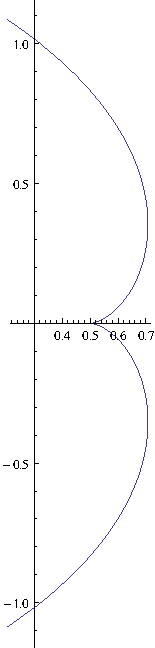
\includegraphics[height=0.4\textheight]{zyklo.pdf}
		\caption{Kaustik}
		\label{fig:zyklo}
	\end{minipage}
	\begin{minipage}[b]{0.6\textwidth}
		\centering
		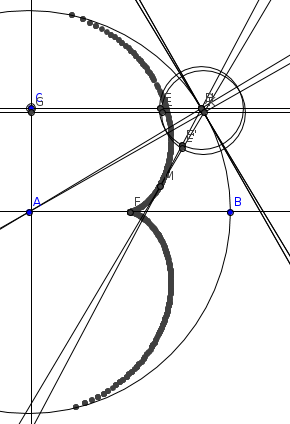
\includegraphics[height=0.4\textheight]{geogebra.png}
		\caption{Spurkurve der lokalen Brennpunkte}
		\label{fig:geo}
	\end{minipage}
\end{figure}

%%%%%%%%%%%%%%%%%%%%%%%%%%%%%%%%%%%%%%%%%%%%%%%%%%%%%%%%%%%%%%%%%%%%%%%%%%%%%%%
%                            Davis-Cotton-Teleskop                            %
%%%%%%%%%%%%%%%%%%%%%%%%%%%%%%%%%%%%%%%%%%%%%%%%%%%%%%%%%%%%%%%%%%%%%%%%%%%%%%%

\section{Davis-Cotton-Teleskop}
\label{3}

\subsection{Brennfleck}

Letztlich muss ich die Geradengleichung aus Aufgabe \ref 2 $H = D/2$ einsetzen
und die Gleichung gleich $0$ setzen und nach $Y$ umstellen.

\fehlt

\subsection{Spiegelparameter}

Wie in Aufgabe \ref 4 gezeigt, fängt ein Paraboloid paralleles Licht in einem
Brennpunkt ein. Also sollte die Fläche $F$ ein Paraboloid (Parabel im Schnitt)
sein. Außerdem sollte $\Psi$ gerade so gewählt werden, dass die Spiegel genau
tangential auf der Parabel liegen. Für infinitesimale kleine Spiegel würde dann
eine perfekte Bündelung auf den Sensor eintreten.

In Aufgabe \ref 4 wird die Funktion für die Parabel hergeleitet:
\[
	y(x) = \frac{x^2 + b^2}{2b}
\]

Dabei ist $b$ der Abstand zwischen Brennpunkt und Koordinatenursprung. Die
Parabel ist allerdings für $x = 0$ nicht 0, also $y(0) \neq 0$. In der Skizze
zum Teleskop ist $f$ allerdings der Abstand zwischen $y(0)$ und dem Brennpunkt.
Also setze ich $b = 2f$ als neue Brennweite ein. Außerdem verschiebe ich um $f$
nach hinten. Somit vereinfacht sich die Parabelgleichung zu:
\[
	y(x) = \frac{x^2}{4f}
\]

Der Winkel $\Psi$ sollte gerade die Ableitung der Parabel sein, es gilt also:
\[
	\Psi = \arctan\del{\frac 12 \frac xf}
\]

Aus der Abbildung auf dem Aufgabenblatt kann ich ablesen:
\[
	\cos\del\theta = \frac{f-y(x)}f
\]

Einsetzen der Funktion $y$ und Umformen nach $x$ liefert:
\[
	x = 2 f \sqrt{1 - \cos\del\theta}
\]

Also ist der Winkel:
\[
	\Psi(\theta) = \arctan\del{\sqrt{1 - \cos\del\theta}}
\]

Die Funktion $\Psi$ hängt nicht von der Brennweite $f$ ab, was zu erwarten ist,
weil das Teleskop vergrößert und verkleinert werden kann, ohne dass sich die
Geometrie ändert. Außerdem gilt $\Psi\del 0 = 0$. Der zentrale Spiegel liegt in
der Tat so, dass er das Licht in den Brennpunkt schickt (wenn nicht der
Detektor im Weg wäre). Und es gilt $\Psi\del{\pi/2} = \pi/4$. Licht, dass
senkrecht zur Einfallsrichtung auf den Detektor trifft, wurde somit richtig
abgelenkt.

\subsection{Schrumpffaktor}

Da die einzelnen Spiegel ideal angeordnet sind, ist nur noch die Streuung durch
die einzelnen Spiegel relevant. Daher kann ich die Formel aus der ersten
Teilaufgabe benutzen und $D$ durch $d$ ersetzen. Das ganze unterscheidet sich
dann in einem Faktor $D^3/d^3$.

%%%%%%%%%%%%%%%%%%%%%%%%%%%%%%%%%%%%%%%%%%%%%%%%%%%%%%%%%%%%%%%%%%%%%%%%%%%%%%%
%                               Parabolspiegel                                %
%%%%%%%%%%%%%%%%%%%%%%%%%%%%%%%%%%%%%%%%%%%%%%%%%%%%%%%%%%%%%%%%%%%%%%%%%%%%%%%

\section{Parabolspiegel}
\label{4}

Ich betrachte eine Funktion $y$. Der Brennpunkt sei an dem Punkt $(0, f)^T$.
Die Strahlen kommen in Phase von einer Ebene, die $h$ über $x$-Achse liegt.
Damit die komplette Wellenfront gleichzeitig ankommt, muss der Weg für jedes
$x$ gleich sein. Dieser Weg soll gerade $C$ sein. Der Weg setzt sich aus dem
Teil, den das Licht senkrecht fällt, und das es nach der Reflexion noch läuft,
zusammen:
\[
	C = (h-y) + \sqrt{x^2 + (f-y)^2}
\]

Dabei wähle ich $C$ so, dass $C - h=0$ erfüllt ist. Somit kann ich umformen:
\begin{align*}
	-y &= \sqrt{x^2 + (f-y)^2} \\
	y^2 &= x^2 + (f-y)^2 \\
	y^2 &= x^2 + f^2 - 2fy + y^2 \\
	2fy &= x^2 + f^2 \\
	  y &= \frac{x^2 + f^2}{2f}
\end{align*}

\begin{figure}
	\centering
	\includegraphics[width=0.5\textwidth]{16-Plot.pdf}
	\caption{Plot der Parabel für $f = 0.5, 1.5, 2.5, 3.5$. Je kleiner das $f$, desto tiefer $y(0)$.}
	\label{fig:}
\end{figure}

Dies ist in der Tat die Gleichung einer Parabel. Diese kann natürlich noch um
eine additive Konstante verschoben werden, in dem man das $C$ anders wählt.
Wenn ich $x$ durch $\rho$ (Zylinderkoordinaten) ersetze, kommt
ein rotationssymmetrischer Paraboloid heraus.

%\bibliography{../../zentrale_BibTeX/Central}
%\bibliographystyle{plain}

\end{document}

% vim: spell spelllang=de
